\chapter{Diseño del Sistema y Decisiones Técnicas}
\label{cap:disenoSistema}

En este capítulo se detallan las decisiones técnicas adoptadas para la implementación de ClimbIt
así como la justificación de dichas elecciones frente a las alternativas existentes. 
También se detallarán las arquitecturas del frontend y del backend y los patrones de diseño 
utilizados.

\section{Diseño del Sistema}
Como se observa en la Figura \ref{fig:diagrama_arquitectura_climbit}, la arquitectura del sistema ClimbIt se estructura bajo un modelo cliente-servidor de tres capas. El flujo de información se inicia en los clientes web y móviles, cuyo tráfico es redirigido  a través de un túnel de Cloudflare que asegura la red local del servidor frente a intrusiones externas. En el servidor, Nginx actúa como \textit{reverse proxy} para servir los recursos del frontend, mientras que una API REST desarrollada en Node.js gestiona la lógica de negocio y el procesamiento de peticiones. Finalmente, la persistencia de la información se delega en un sistema de gestión de bases de datos PostgreSQL supervisado mediante la herramienta gráfica PgAdmin,  garantizando así una infraestructura robusta, escalable y con una clara separación de responsabilidades. Todo el sistema se encuentra alojado en una Raspberry Pi 4 en diferentes contenedores Docker. La explicación detallada de cada una de las capas y los componentes que las conforman se encuentra en la sección \textit{Integración Continua, Despliegue y DevOps}
 
\begin{figure}[!h]
    \centering
    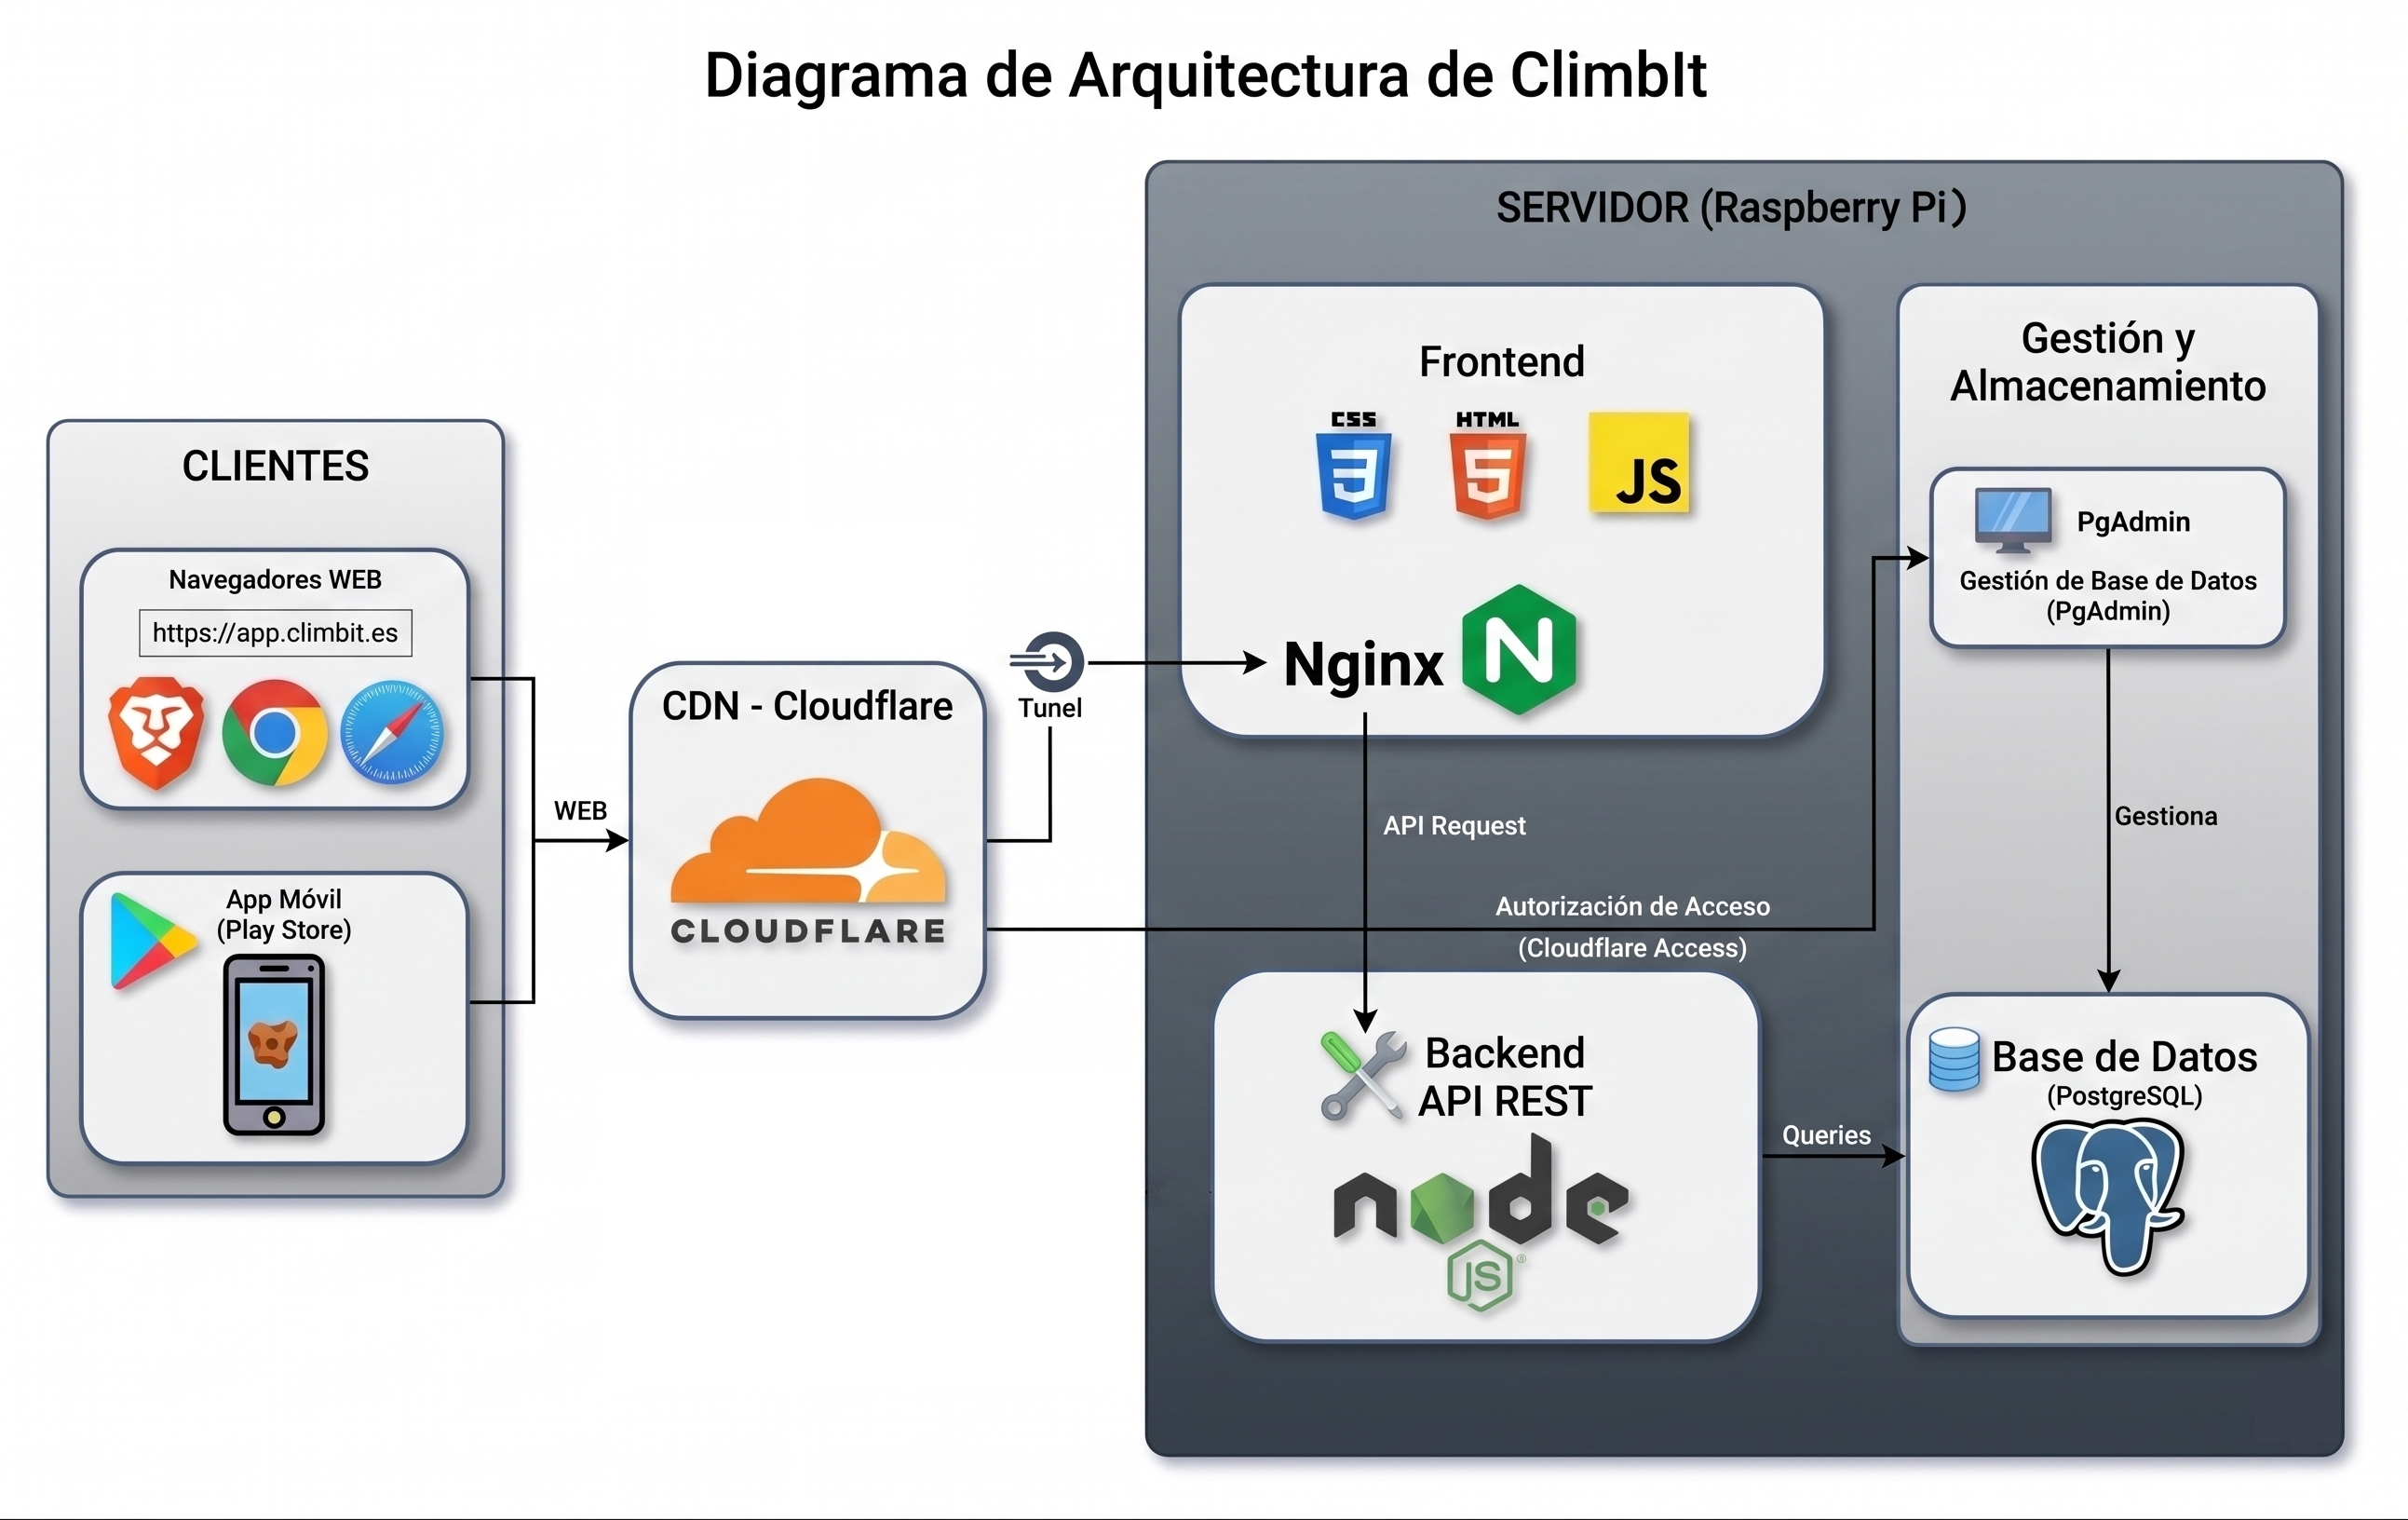
\includegraphics[width=1\textwidth]{./Imagenes/Fuentes/DiagramaArquitecturaClimbIt.png} 
    \caption{Diagrama de la arquitectura del sistema ClimbIt}
    \label{fig:diagrama_arquitectura_climbit}
\end{figure}

A continuación, se detallan las decisiones de diseño y el stack tecnológico utilizado para cada una de las capas del sistema, así como la arquitectura y los patrones de diseño implementados tanto en el backend como en el frontend.

\section{Decisiones de Diseño y Stack Tecnológico}

Para cumplir con los requisitos marcados para ClimbIt se determinó que un modelo cliente-servidor era la mejor opción para mantener la separación de responsabilidades: lógica de negocio y persistencia de los datos en el backend y un frontend SPA (\textit{Single Page Application}) simple y de fácil navegación que consuma esos datos a través de una API.Tras un análisis inicial del alcance del proyecto se llegó a la conclusión de que era notablemente amplio, por lo que la decisión sobre qué arquitectura utilizar fue ampliamente meditada. Valoramos tres opciones de diseño para el backend: una \textbf{arquitectura monolítica}, una \textbf{arquitectura hexagonal} y una arquitectura basada en \textbf{microservicios}. 

Para la elección tuvimos en cuenta tres factores principales: \textbf{escalabilidad}, \textbf{mantenibilidad} y  \textbf{complejidad de desarrollo}. Una arquitectura monolítica podría haber sido más sencilla de implementar inicialmente, pero a medida que el proyecto creciese y la posibilidad de que los requisitos cambiasen, podría habernos llevado a un código difícil de mantener y escalar. Por otro lado, una arquitectura de microservicios habría ofrecido grandes ventajas en cuanto a la escalabilidad en el largo plazo, pero su empinada curva de aprendizaje, la dificultad que añadía al desarrollo y la necesidad de gestionar múltiples servicios sumada a la prácticamente nula necesidad para la implementación los requisitos funcionales marcados para el alcance del proyecto hizo que fuera la primera en ser descartada. Al final decidimos que la arquitectura hexagonal nos daba el equilibrio entre dificultad de desarrollo, mantenibilidad y escalabilidad que buscábamos para ClimbIt, permitiéndonos desacoplar toda la lógica de negocio de factores externos como la base de datos y el frontend, quedando así un sistema más modular y fácil de mantener a largo plazo.

En cuanto al stack tecnológico, para el backend se optó por usar \textbf{Node.js} con \textbf{Express} debido a su popularidad, fiabilidad y amplio ecosistema de librerías, así como la extensa documentación disponible. Como lenguaje de programación se decidió trabajar directamente con \textbf{JavaScript} en formato ESModules y no con TypeScript principalmente porque Node.js no tiene un soporte completo para todas las funcionalidades que ofrece TypeScript.

Para la base de datos, se descartó desde el principio las bases de datos no relacionales, ya que la naturaleza de los datos de ClimbIt, con relaciones claras entre escaladores, rocódromos y rutas, se adaptaba mejor a un modelo relacional. \textbf{PostgreSQL} se ha convertido en la base de datos relacional más utilizada y querida en el mundo del desarrollo, como se demuestra en la encuesta anual \textit{Stack Overflow Developer Survey}\footnote{https://survey.stackoverflow.co/2025/technology\#most-popular-technologies-database-database-prof} del pasado año 2025, debido a su gran rendimiento, escalabilidad y comunidad. Otras opciones como MySQL o MariaDB también eran opciones válidas, pero al no ofrecer características como soporte nativo para tipos de datos JSON o arrays, que sí ofrece PostgreSQL, y que se adaptaban perfectamente a las necesidades del proyecto, se decidió que PostgreSQL era la mejor opción.

Para la comunicación entre el backend y la base de datos, se decidió que utilizar un ORM (\textit{Object-Relational Mapping}) facilitaria el desarrollo y colocaría una capa extra de seguridad. Después de evaluar varias opciones se determinó que \textbf{Sequelize}, debido a su diseño nativo para JavaScript, era la opción más indicada. Otros ORMs como TypeORM o Prisma también barajaron, pero al estar orientados a TypeScript no se podría aprovechar al máximo sus características.

A la hora de servir imágenes al frontend, se llegó a la conclusión de que tener imágenes sin procesar en el servidor jugaría en nuestra contra a la hora de tener un buen rendimiento, por lo que decidimos generalizar el uso del formato \textbf{webp} en todas las imágenes que se subieran a la aplicación, exceptuando los mapas de las zonas, que se mantendrían en formato \textbf{svg}. Obligar a que los usuarios subieran las imágenes en un único formato generaría una gran fricción a la hora de usar la app, por lo que la solución más óptima era permitir una amplia gama de formatos para las imágenes y convertirlas en el servidor antes de almacenarlas. Para esta tarea se optó por utilizar la librería \textbf{ffmpeg}, una de las librerías más populares y potentes para el procesamiento de imágenes.

En cuanto a la gestión de sesiones, se decidió usar \textbf{JWT} (\textit{JSON Web Tokens}) por su ligereza y capacidad de escala. Los tokens contienen la información necesaria sobre permisos e identidad del usuario, eliminando la necesidad de realizar validaciones completas con cada petición y mejorando así los tiempos de respuesta y el rendimiento. Además, al estar firmados con una clave secreta, se garantiza que los datos no pueden ser manipulados, proporcionando una capa adicional de seguridad sin cargar el servidor con sesiones almacenadas.

Para el frontend se planteó desde el principio la necesidad de que la aplicación tuviera que ser utilizada desde dispositivos móviles, pero no se quería limitar el uso a un tipo de dispositivo concreto, ya que supondría perder una amplia base de usuarios. Por lo que se debía decidir entre desarrollar aplicaciones nativas para cada plataforma, lo que supondría un esfuerzo inasumible para el alcance del proyecto, o desarrollar una aplicación web, pero que permitiese utilizarla como si fuera nativa. La decisión estaba clara, se optó por desarrollar una \textbf{PWA} (\textit{Progressive Web App}), que permitía tener la flexibilidad y alcance para que cualquier usuario, independientemente de su dispositivo, pudiera acceder a la aplicación.

Para desarrollar la aplicación, después de valorar las ventajas que nos ofrecían distintos frameworks frente a la curva de aprendizaje y la complejidad añadida que suponían, decidimos optar por una solución más ligera y sencilla: utilizar \textbf{HTML}, \textbf{CSS} y \textbf{JavaScript} puro junto con \textbf{Bootstrap} para mantener un diseño consistente. Esta decisión permitía mantener un control total sobre el código y a la vez que una velocidad inicial de desarrollo  mayor debido a los conocimientos previos. Por otro lado, sí suponía un reto la implementación de ciertas funcionalidades, en concreto el enrutamiento de las vistas o la implementación manual de componentes personalizados, que es algo que los frameworks manejan de forma nativa y que se tenían que implementar desde cero.


\section{Diseño de la Arquitectura}

\subsection{Backend}
(Pendiente de refactorización)
Una vez elegida la arquitectura hexagonal para el backend, se diseñó la estructura del proyecto siguiendo los principios de 
esta arquitectura y aplicando una serie de patrones de diseño que nos permitieran mantener un código limpio, sencillo y modular, 
completamente independiente entre las diferentes capas. La arquitectura hexagonal organiza el código en capas definidas, 
donde cada una tiene una responsabilidad clara. La capa de dominio se encarga de la lógica de negocio y las reglas del sistema, 
donde se definen todos los contratos y validaciones sobre los objetos que se procesan. La capa de infraestructura se encarga
de la comunicación con la base de datos, que nosotros gestionamos a través de Sequelize, así como los modelos que representan
las entidades del sistema, las migraciones y las seeds. La capa de aplicación se encarga de definir la lógica de los  casos de uso, orquestando la interacción entre la capa de dominio y la capa de infraestructura. Por último, la capa de presentación, 
que nosotros hemos llamado interfaz, se encarga de la comunicación con el frontend a través de una API REST, definiendo los 
endpoints, los controladores que gestionan las peticiones y respuestas y los middlewares que nos ayudan a la autenticación 
de tokens, formatos de datos y validaciones tanto de datos como de archivos.

{Diagrama de la arquitectura hexagonal del backend con ejemplo de ClimbIt}

A lo largo del desarrollo nos encontramos con diversas situaciones que nos llevaron a aplicar diferentes patrones de diseño que 
nos ayudaron a obtener un código más limpio, modular y fácil de mantener. Los patrones de diseño que hemos utilizado son los siguientes:

\paragraph{Patrón Repository:} Este patrón propuesto por Martin Fowler consiste en crear una interfaz entre la lógica de negocio y la capa
de persistencia, en nuestro caso, nuestra base de datos PostgreSQL a través de Sequelize, de manera que nos permite desacoplar el negocio
de la infraestructura, manteniendo así un código más mantenible en el tiempo. En nuestro caso, como se puede ver en la \ref{fig:diagrama_repository},
la capa de dominio define la interfaz del repositorio en la que se establecen los métodos que se necesitan para realizar las diferentes operaciones
y la capa de infraestructura implementa dicha interfaz con la que hablar con la base de datos. De esta manera, la capa de aplicación
solo se encarga de definir la lógica de los distintos casos de uso.

\begin{figure}[!h]
    \centering
    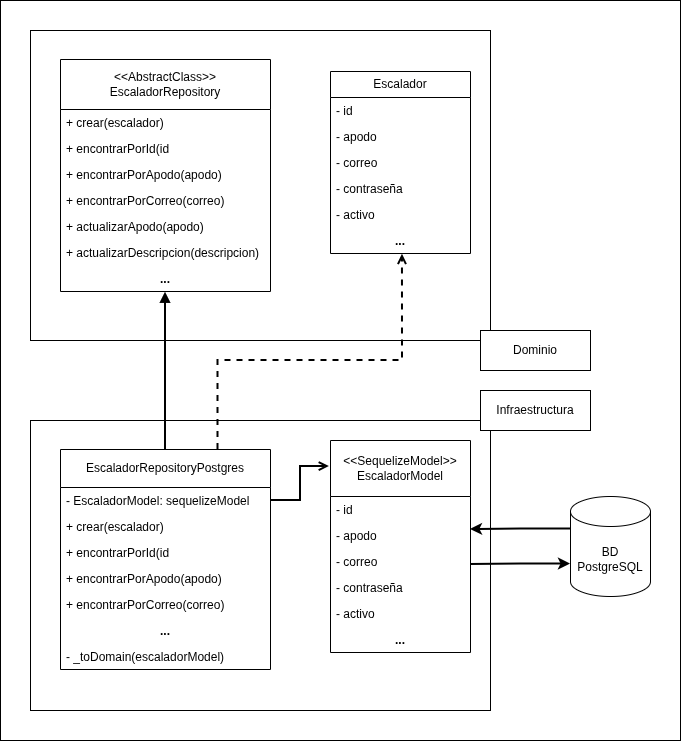
\includegraphics[width=1\textwidth]{./Imagenes/Fuentes/Diagrama_Patron_Repository.png} 
    \caption{Diagrama patrón Repository en ClimbIt}
    \label{fig:diagrama_repository}
\end{figure}

\paragraph{Patrón Adapter:} El patrón Adapter es uno de los patrones clásicos introducidos por Erich Gamma, Richard Helm, Ralph Johnson y John Vlissides, 
también conocidos como los ``Gang of Four'' y se encarga de adaptar distintas interfaces para que puedan trabajar entre ellas. En nuestro caso,
lo hemos utilizado para adaptar distintos errores que pueden surgir en las diferentes capas, como se puede observar en la \ref{fig:diagrama_adapter}, para 
centralizar el manejo de estos errores en un único lugar, permitiéndonos así mantener una consistencia a la hora de tratar los distintos 
errores que pueden surgir.


\begin{figure}[h]
    \centering
    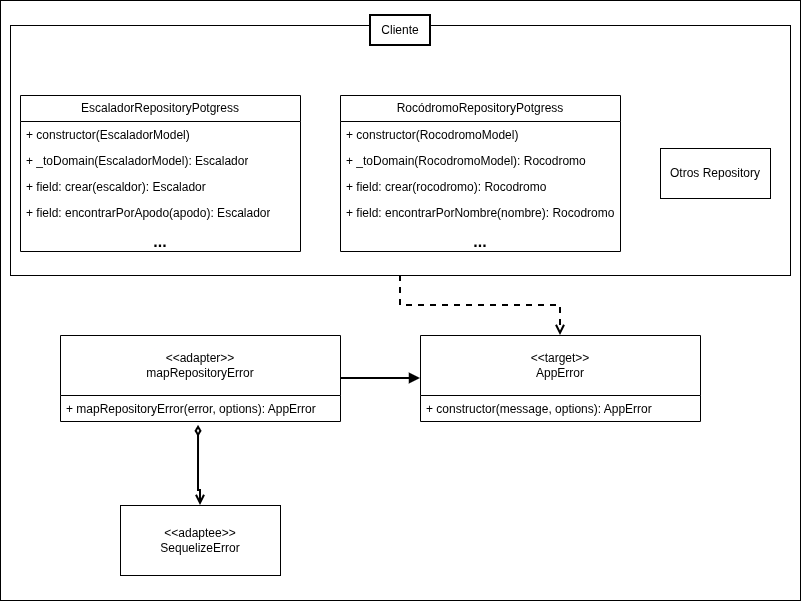
\includegraphics[width=1\textwidth]{./Imagenes/Fuentes/Diagrama_Patron_Adapter.png} 
    \caption{Diagrama patrón Adapter en ClimbIt}
    \label{fig:diagrama_adapter}
\end{figure}

\paragraph{Patrón Singleton:} Introducido también por ``The Gang of Four'' en su libro ``Design Patterns: Elements of Reusable Object-Oriented Software'', 
el patrón Singleton sirve para garantizar que una clase tenga únicamente una instancia al mismo tiempo a lo largo de la ejecución de la aplicación. 
En nuestro caso, lo hemos utilizado, por ejemplo, para mantener una única conexión a la base de datos, evitando así posibles problemas y errores relacionados
con múltiples conexiones abiertas, pero también lo hemos utilizado en otros puntos que detallaremos más adelante en la implementación de la aplicación.

\paragraph{Inyección de dependencias e Inversión de control:} La inversión de control es un principio abstracto popularizado por Robert C. Martin, también conocido 
como ``Uncle Bob'', pero ideada inicialmente por Martin Fowler, que viene a referir que los objetos no deben crear sus propias dependencias, sino que le tienen
que venir dadas de fuera. Por otro lado, la inyección de dependencias es una de las técnicas para implementar este principio. En nuestra aplicación hemos
utilizado la inyección de dependencias a través de la inyección por constructor transversalmente en toda la aplicación. El controlador recibe por inyección
los casos de uso que necesita para gestionar las peticiones, los use cases reciben por inyección los repositorios que necesitan para realizar sus operaciones 
y los repositorios reciben por inyección los modelos que necesitan para hablar con la base de datos. De esta manera, hemos conseguido un código completamente desacoplado
alineado con la filosofía de la arquitectura hexagonal.

\subsection{Frontend}

Como se describe en la sección anterior, la arquitectura del frontend fue diseñada adoptando una aproximación modular 
y por capas sin usar frameworks tradicionales como React o Vue, lo que implicó implementar manualmente ciertos patrones 
como el enrutado de vistas y la gestión del ciclo de vida de componentes. Esta decisión se justificaba por la necesidad 
de mantener un control total sobre el código y maximizar la velocidad inicial de desarrollo.

\paragraph{Arquitectura en Capas:} La estructura del frontend se organiza en tres capas claramente diferenciadas:

\begin{itemize}
    \item \textbf{Capa Core:} Centraliza toda la lógica de infraestructura transversal, incluyendo el cliente HTTP centralizado que gestiona la comunicación con la API REST del backend, la inyección automática de tokens JWT, el manejo de errores para situaciones offline, y el enrutado por hash que controla la navegación entre vistas. Esta capa también incluye utilidades globales de UI como el banner de conectividad, estados de carga y manejo de formularios.
    
    \item \textbf{Capa Modules:} Agrupa el código de negocio por dominios funcionales (autenticación, escalador, rocódromo, ruta, zona, social, error). Cada módulo sigue el patrón controlador-vista, donde el controlador orquesta la obtención de datos del cliente HTTP centralizado y controla el flujo de interacción, mientras que la vista se encarga únicamente del renderizado HTML y el enlace de callbacks de eventos. Este patrón establece una separación clara de responsabilidades: la vista no contiene lógica de negocio, y el controlador no contiene lógica de presentación.
    
    \item \textbf{Capa Components:} Alberga todas las piezas reutilizables de interfaz. De esta forma, se logra reducir la duplicidad y se mantiene una consistencia visual a lo largo de toda la app: barra de navegación, formularios editables, modales de confirmación, notificaciones toast, selectores de imágenes, mapas SVG interactivos con pan y zoom, tarjetas de estadísticas de progreso y botones de estado. Cada componente expone funciones de renderizado que generan HTML y funciones de inicialización que vinculan listeners de eventos.
\end{itemize}

\paragraph{Arquitectura Controlador-Vista:} Originalmente, se planteó la implementación del frontend con el patrón MVC(Modelo-Vista-Controlador), pero se optó por unificar Modelo y Controlador, ya que la lógica de negocio se encuentra toda delegada al backend y significaría añadir una capa extra que no aportaría tanto valor en contraposición a la complejidad extra que implicaría. Por ello, se adoptó esta simplificación en la que el controlador se encarga de realizar las llamadas a la API a través del cliente HTTP y procesa los datos obtenidos para usarlos en la vista, que se encarga de renderizar el contenido. El controlador y la vista tienen unas funciones bien diferenciadas:
El controlador es responsable de:

\begin{itemize}
    \item Llamadas a la API a través del cliente HTTP para obtener y enviar datos.
    \item Procesar los datos obtenidos del backend para su uso en la vista.
    \item Procesar los datos recibidos de la vista para enviarlos al backend.
    \item Gestionar el estado local del módulo (almacenado en variables de módulo o \texttt{localStorage}).
    \item Construir el contexto necesario para renderizar la vista(construcción de componentes, preparación de datos...).
    \item Definir callbacks que respondan a los eventos que se sucedan en la vista por parte del usuario.
\end{itemize}

La vista, por su parte, se encarga únicamente de:

\begin{itemize}
    \item Generar el HTML necesario basado en los datos proporcionados por el controlador.
    \item Enlazar listeners de eventos a elementos del DOM.
    \item Delegar todos los eventos de usuario a los callbacks del controlador.
\end{itemize}

Esta división reduce el acoplamiento, facilita la comprensión del código y permite una mejor escalabilidad y mantenimiento del proyecto.

\paragraph{Cliente HTTP:} Similar al patrón Repository en el backend, el cliente HTTP actúa como único mediador entre los módulos y la API REST. Sus responsabilidades son: la inyección del token JWT en los headers de autenticación, la detección de respuestas 401 (sesiones expiradas) que dispara el borrado del token y redirecciona al login, y  marcar el comportamiento cuando no hay conexión a red. En modo offline, el cliente distingue entre operaciones de solo lectura (GET, HEAD) que pueden proceder con datos en caché, y operaciones de escritura (POST, PUT, DELETE) que son rechazadas, asegurando que el usuario pueda seguir consultando la información almacenada sin poder realizar cambios que no puedan ser sincronizados con el servidor.

\paragraph{PWA y Estrategia de Caché:} La aplicación se encuentra completamente diseñada e implementada como una PWA. 
En el manifiesto se definen  el modo \texttt{standalone} para que la aplicación se comporte como una app nativa instalada, la orientación se bloquea 
a portrait cuando se ejecuta en modo instalado, y se establece un ícono y tema de color consistentes.
En el service worker se establecen una serie de características para garantizar una experiencia fluida para el usuario, 
tanto online como offline. A través de la librería Workbox, se han implementado estrategias de caché para cada tipo de recurso en función de los criterios que se han considerado más relevantes en su impacto a la experiencia del usuario.
Las distintas estrategias de caché son las siguientes, organizadas por tipo de recurso:

\begin{itemize}
    \item \textbf{Librerías externas} (CDN de Bootstrap, Material Icons, etc.): Caché-first con expiración anual, priorizando velocidad, ya que estos recursos cambian raramente.
    
    \item \textbf{Imágenes de rutas:} Stale-while-revalidate con expiración de 20 minutos, permitiendo que se sirvan versiones en caché mientras se actualizan en segundo plano, mejorando la respuesta inicial sin sacrificar frescura.
    
    \item \textbf{APIs de negocio} (endpoints de escaladores, rocódromos, zonas, rutas): Network-first con timeout de 10 segundos, priorizando datos frescos pero cayendo a caché si la red tarda o no está disponible.
    
    \item \textbf{Activos de interfaz} (logos, avatares): Stale-while-revalidate con expiración de 1 día, proporcionando una buena     experiencia visual incluso en conexiones lentas.
\end{itemize}

Esta diferenciación en la caché asegura que la experiencia offline sea funcional para consultar tus estadísticas o las rutas de un rocódromo, mientras que la estrategia de caché en línea minimiza tiempos de respuesta sin sacrificar sustancialmente la consistencia de datos.

\section{Diseño de la Base de Datos}

Como se mencionó anteriormente en la sección de decisiones tecnológicas, la naturaleza de los datos en ClimbIt presentaba 
relaciones claras y bien definidas entre las diferentes entidades, desglosadas en el siguiente punto. Esto propició que se
descartara desde el principio las bases de datos no relacionales en favor de un modelo relacional. La estructura jerárquica 
y las múltiples relaciones muchos-a-muchos, como se representa en la Figura XX, entre entidades hacían que un modelo relacional fuese la opción más apropiada 
para garantizar integridad referencial, coherencia de datos y facilidad de consultas complejas.

PostgreSQL fue el sistema gestor de bases de datos relacional (SGBDR) que mejor se adaptaba a los requerimientos del proyecto debido
a su robustez, rendimiento, escalabilidad y su creciente popularidad en el ecosistema de desarrollo. Para facilitar la interacción 
entre la aplicación y la base de datos, utilizamos Sequelize como ORM, que nos permite trabajar con los modelos de datos de forma 
orientada a objetos sin necesidad de escribir SQL directamente, proporcionando además una capa adicional de seguridad contra 
inyecciones SQL y abstrayendo las particularidades específicas de PostgreSQL.

\subsection{Entidades Principales del Sistema}

Tras el análisis de los datos obtenidos en las capturas de requisitos y el modelado de las Historias de Usuario que se 
implementarían, el modelo de datos de ClimbIt quedó compuesto por las entidades y relaciones que se pueden ver en
la Figura XX. Las entidades principales son las siguientes:

{ Figura del modelo E-R }

\begin{itemize}
    \item \textbf{Escalador:} Representa a los usuarios del sistema. En ella se almacena la información de perfil (apodo, descripción),
    credenciales de autenticación (email, contraseña) y configuración personal.
    
    \item \textbf{Rocódromo:} Entidad que representa cada uno de los lugares donde se practica la escalada, incluyendo configuración de dificultades
    para ese rocódromo e información como nombre, ubicación, descripción y horarios.
    
    \item \textbf{Zona:} Las diferentes áreas dentro de un rocódromo, cada una con su propio mapa e información propia.
    
    \item \textbf{Pista:} Las rutas específicas de escalada dentro de una zona, con información de dificultad, tipo de escalada y la zona del rocódromo
    de la que forman parte. 
    
    \item \textbf{EscalaDificultad:} Tabla de catálogo que define los niveles de dificultad disponibles en el sistema.
    
    \item \textbf{FotosPerfil:} Almacenamiento de url de imágenes de perfil disponibles para los escaladores.
\end{itemize}

\subsection{Relaciones Principales del Modelo}

El modelo relacional de ClimbIt está estructurado mediante las siguientes relaciones:

\paragraph{Relaciones Jerárquicas:} La estructura principal del sistema sigue una jerarquía clara:
\begin{itemize}
    \item Un \textbf{Rocódromo} contiene múltiples \textbf{Zonas} (relación 1:N).
     
    \item Una \textbf{Zona} contiene múltiples \textbf{Pistas} (relación 1:N).
     
    \item Una \textbf{Foto de Perfil} puede ser utilizada por múltiples \textbf{Escaladores} (relación 1:N).
     
    \item Una \textbf{Escala de Dificultad} puede ser utilizada por múltiples \textbf{Rocódromos}, pero un \textbf{Rocódromo} solo puede tener 2 \textbf{Escalas de Dificultad} diferentes,
    una para vías y una para bloque (relación 2:N).
\end{itemize}

\paragraph{Relaciones Muchos-a-Muchos:} El sistema implementa varias relaciones M:N que se representan a través de las siguientes tablas de unión:
\begin{itemize}
    \item \textbf{Escalador-Escalador} a través de \textit{SolicitudAmistad}. Un escalador puede solicitar amistad a otro, representados en esta tabla como 
    \textit{Remitente} y \textit{Destinatario}.

    \item \textbf{Escalador-Escalador} a través de \textit{Amistad}. Se gestionan las amistades entre dos usuarios que establezcan tras aceptar
    las solicitudes de la tabla \textit{SolicitudAmistad}.

    \item \textbf{Escalador-Rocódromo} a través de \textit{Suscripción}, permite a un escalador suscribirse a múltiples rocódromos y viceversa, que un rocódromo
    tenga múltiples suscriptores.

    \item \textbf{Escalador-Rocódromo} a traves de \textit{GestorRocódromo}, que contiene a los escaladores que tienen permiso de gestión de los rocódromos existentes, 
    permitiendo que un rocódromo tenga múltiples gestores y que un escalador pueda gestionar múltiples rocódromos.

    \item \textbf{Escalador-Pista} a través de \textit{EscalaPista}, registrando cada ascenso realizado o como proyecto de hacerlo por cada escalador.
\end{itemize}

\subsection{Normalización y Diseño}

La estructura de la base de datos ha sido diseñada siguiendo los principios de normalización relacional, alcanzando 
la tercera forma normal (3FN) en la mayoría de las entidades. Esto implica:

\begin{itemize}
    \item Eliminación de datos redundantes, evitando la duplicación de información.
    \item Cada atributo depende únicamente de la clave primaria de su entidad.
    \item Separación de conceptos en entidades distintas con relaciones apropiadas entre ellas.
\end{itemize}

Estas prácticas de normalización garantizan que las operaciones de actualización, inserción y eliminación sean eficientes 
y no generen inconsistencias en los datos.

La tabla de \textit{EscalasDificultad} es la única que no cumple la 3FN. Esta tabla incluye un campo \textit{Dificultades} de tipo array que almacena todos los niveles
de dificultad, rompiendo el principio de atomicidad. Esta decisión se tomó para mejorar el proceso de obtención de las dificultades disponibles en cada rocódromo, 
evitando así la necesidad de realizar consultas adicionales a la hora de crear una ruta. PostgreSQL ofrece el uso de estos tipos de datos de forma nativa, 
por lo que se decidió que almacenar las dificultades de esta forma era lo más óptimo para el rendimiento de la aplicación.

\subsection{Decisiones de Diseño Específicas}

A lo largo del diseño de la base de datos se tomaron varias decisiones específicas:

\paragraph{Campos de Estado y Booleanos:} Se utilizan campos booleanos para representar estados como \texttt{Activo} en todas las entidades principales. Esto permite
realizar borrados lógicos en entidades sin eliminarlas completamente, facilitando así el mantenimiento histórico de datos y la consistencia entre relaciones. También
se han utilizado como sustitutos de roles específicos, concretamente en el caso de los gestores, se encuentra el campo \textit{Propietario}, que es un booleano para indicar 
si ese gestor además es propietario, que en el futuro que se especifica en la sección de Conclusiones y Trabajo Futuro, le otorgará permisos adicionales. Lo mismo 
sucede con el campo \textit{isAdmin} en la tabla de escaladores, que indica si un usuario tiene permisos de administrador o no, lo que le otorgará permisos adicionales
a la hora de gestionar puntos clave de ClimbIt.

\paragraph{URLs y Rutas de Imágenes:} Campos como \textit{logoURL}, \textit{imagenURL} y \textit{mapa} almacenan 
rutas a los recursos asociados a cada entidad. Las imágenes se almacenan en el servidor tras ser procesadas 
a formato webp y se guardan en sendos campos la ruta relativa a ese recurso.

\paragraph{Timestamps:} Cada entidad cuenta con campos autogenerados por PostgreSQL: \textit{CreatedAt}, fecha en al que se creó la entrada de ese
recurso en la base de datos, y  \textit{UpdatedAt}, que se actualiza cada vez que ese recurso sufre algún tipo de modificación Estos campos permiten llevar una 
trazabilidad para cada recurso y su utilización dentro del sistema para servirla como información al usuario en puntos relevantes, como por ejemplo en las Pistas, 
indicándole cuando fue su introducción al rocódromo.

\paragraph{Enumeraciones:} Ciertos campos utilizan tipos enumerados. En la tabla \textit{EscalaPista} se utiliza en el campo \textit{Estado}, que contiene los estados  (completado, intentando, etc.) 
en los que se puede encontrar el progreso de un escalador con respecto a la ruta: \textit{Flash} si la completo al primer intento, \textit{Completado} si la completó en varios
y \textit{Proyecto} si la quiere marcar para completarla en un futuro. En la tabla \textit{SolicitudAmistad} también se encuentra el campo \textit{Estado}, puede tomar otros 3 
valores: \textit{Pendiente} si la solicitud de amistad ha sido enviada y aún no ha sido gestionada, \textit{Aceptada} si la solicitud se aceptó y se inició una amistad 
y \textit{Rechazada} si el destinatario la rechazó. Por último, en la tabla \textit{Pista}, se encuentra el campo \textit{Tipo}, que puede tomar los valores de 
\textit{Bloque} o \textit{Vía}, dependiendo del tipo de pista que se esté dando de alta.

\subsection{Migraciones y Seeders:}

Toda la estructura de la base de datos se gestiona a través de migraciones controladas por Sequelize, permitiendo:

\begin{itemize}
    \item Versionado de cambios en el esquema de la base de datos.
    \item Posibilidad de revertir cambios si es necesario.
    \item Reestructuración y repoblado de tablas en actualizaciones de esquema.
    \item Documentación implícita de la evolución del modelo de datos.
    \item Reproducibilidad del esquema en diferentes entornos (desarrollo, pruebas, producción).
\end{itemize}

Adicionalmente, se utilizaron \textit{seeders} al principio del desarrollo para poblar la base de datos con datos de prueba, para realizar tests y comprobaciones, 
pero se cambió posteriormente a poblados mediante Postman, ya que permite una gran flexibilidad, rapidez y facilita incluso la subida de imágenes.

\section{Diseño de la UI y UX}

A lo largo de esta sección se detalla el proceso de diseño de la interfaz y la experiencia de usuario (UI/UX) de la aplicación. El objetivo principal es plasmar los requisitos obtenidos en el proceso de captura de requisitos y las necesidades específicas identificadas en una solución visual que sea intuitiva y eficiente. ClimbIt se diseñó bajo la idea principal de ser simple y fácil de usar para cualquier tipo de usuario. Para ello, se optó por diseñar una interfaz limpia, con una jerarquía clara y un flujo de navegación que guíe al usuario de forma natural adoptando para ello conceptos e ideas ya establecidas para obtener una experiencia fluida y consistente con aplicaciones ya existentes.

\subsection{Arquitectura de la información y Flujo de Navegación}

Como puede observarse en \{Diagrama de flujo de ClimbIt\}, la estructura que sigue ClimbIt es una combinación entre una estructura \textit{plana} para las vistas principales y una estructura jerárquica de árbol para las vistas secundarias que nacen de ellas. De esta forma, se garantiza un acceso rápido a todas las funcionalidades principales desde cualquier punto de la raíz de la aplicación, pero manteniendo una disposición organizada del contenido.

La navegación comienza con un flujo lineal de inicio de sesión y registro que actúa como puerta de acceso. Una vez se ha realizado este paso, la aplicación se muestra tres secciones principales: \textbf{Social}, que agrupa las funcionalidades relacionadas con la interacción entre escaladores; \textbf{Mis Rocódromos}, que contiene el contenido principal de la aplicación y es la vista a la que se accede por defecto y \textbf{Perfil}, donde se muestra la información del escalador y sus estadísticas generales con respecto a sus registros en la aplicación. Mientras que estas tres secciones conviven en un mismo nivel jerárquico accesible desde el menú de navegación inferior, cualquier subsección adicional, por ejemplo, el detalle de una \textbf{Ruta} o la \textbf{Información del Rocódromo}, desplaza al usuario hacia niveles inferiores del árbol, donde la navegación se vuelve principalmente vertical para mantener el foco en la tarea que se busca realizar.


\subsection{Disposición de Elementos y Jerarquía Visual}

ClimbIt utiliza un lenguaje visual consistente fundamentado en principios de usabilidad para que el usuario identifique la importancia de los elementos de manera intuitiva. La disposición de los componentes sigue el \textbf{patrón de escaneo en F}, situando los elementos de mayor relevancia informativa, como el logo o el título de la sección, en la zona superior izquierda del \textit{header}.

La jerarquía visual se adapta dinámicamente según la profundidad de la navegación:
\begin{itemize}   
    \item \textbf{Priorización del contenido y Ley de Proximidad:} En las vistas de nivel inferior, el \textit{footer} desaparece para maximizar el área de visualización y dar prioridad al contenido. Los elementos de control a lo largo de la aplicación, como botones de edición de rutas para gestores de rocódromos, se agrupan siguiendo la \textit{Ley de Proximidad de la Gestalt}, lo que permite al usuario entender que los botones de acción  afectan únicamente al objeto contenido en dicha tarjeta.
    
    \item \textbf{Ley de Miller:} En línea con el objetivo de mantener una interfaz simple y limpia, se ha aplicado la \textbf{Ley de Miller} a lo largo de toda la aplicación. Esta ley sugiere que el ser humano solo puede procesar una cantidad limitada de información simultáneamente ($7 \pm 2$ elementos). Por ejemplo, al fragmentar la aplicación en tres secciones principales o mostrar  cuatro botones de estado en las rutas, se minimiza la carga cognitiva y se permite al usuario dominar más rápido la navegación dentro de la app y evitando así la saturación informativa.

    \item \textbf{Efecto Zeigarnik y gamificación:} Como puede apreciarse en la vista de una zona \{imagen de zona\}, la inclusión de una \textit{progress bar} de completitud apela al \textbf{efecto Zeigarnik}. Al mostrar visualmente una tarea como "incompleta", se genera una tensión cognitiva en el usuario que incentiva la motivación extrínseca para finalizar las rutas restantes de la zona y alcanzar el estado de completitud.
    
    \item \textbf{Consistencia en el Control:} El \textit{header} actúa como un ancla de navegación; mientras que en el nivel principal refuerza la identidad de marca, en las subsecciones prioriza la funcionalidad mediante una flecha de retorno siempre situada en el mismo cuadrante, proporcionando un sentido de seguridad y control al usuario profundiza dentro de la jeraquía de árbol de una sección.
     
    \item \textbf{Ley de Fitts y accesibilidad motriz:} Como se observa en la vista de detalle de \textbf{Ruta} 
    \{imagen detalles de ruta\}, las acciones principales de cambio de estado (Flash, Completado, Proyecto y Desmarcar) se han implementado como botones de gran tamaño. Al aumentar el área de contacto y situarlos en la zona central de la pantalla, se reduce el tiempo necesario para realizar la interacción y se minimiza el error de precisión, facilitando su uso incluso en situaciones de fatiga física en las manos tras la escalada.
\end{itemize}

\subsection{Decisiones de Diseño}

En este apartado se detallan las elecciones técnicas y estéticas que dan forma a ClimbIt, justificando el porqué de su implementación frente a otras soluciones de interfaz.

\paragraph{Navegación y Estructura:} Se optó por una barra de navegación inferior (\textit{Bottom Navigation Bar}) para las secciones principales. Esta decisión responde a la necesidad de mantener las funciones de \textbf{Social}, \textbf{Mis Rocódromos} y \textbf{Perfil} siempre al alcance del pulgar, optimizando el uso de la aplicación con una sola mano y manteniendo una consistencia externa con otras aplicaciones móviles similares, reduciendo la curva de aprendizaje y la fricción de uso para el usuario. En contraste, la navegación por secciones secundarias se gestiona verticalmente para guiar al usuario a mantener el foco en la tarea específica y evitar distracciones.

\paragraph{Uso de Cards:} La información de los rocódromos y las rutas se organiza mediante el uso de \textit{cards}. De esta manera podemos unificar los datos relevantes de cada ruta o rocódromo en unidades independientes, ayudando al usuario a procesar la información de manera fragmentada y organizada.

\paragraph{Gestión de estados vacíos:} En vistas como la de \textbf{Mis Rocódromos} y \textbf{Social}, cuando recién se ha registrado un escalador, que no seencuentra suscrito a ningún rocódromo ni ha entablado amistad dentro de la aplicación con otro escalador, se mostrarían vacías. Este hecho es desalentador para los usuarios, ya que se encuentran frente a un lienzo en blanco sin información de que hacer. Para evitarlo, se han implementado vistas específicas para no solo informar del estado, sino también para guiar a los usuarios a realizar la acción deseada, como buscar y suscribirse a un rocódromo o enviar solicitudes de amistad a otros escaladores, fomentando así la interacción con la aplicación.

\paragraph{Uso del Color:} El color predominante en ClimbIt es el naranja, que según la teoría del color, evoca energía,  entusiasmo y vitalidad, aspectos completamente alineados con la escalada. Se ha utilizado como color primario en la aplicación para destacar elementos de acción como los botones, para elementos informativos como la ubicación dentro del menú de navegación o de solicitud de amistad pendiente y para forjar una identidad visual fuerte y coherente en toda la aplicación. El resto de colores de la paleta utilizada han sido colores neutros, como el blanco para los fondos, aportando luminosidad y sensación de espacio, el negro para textos e información principal y el gris para establecer una jerarquía de lectura en textos secundarios e indicar inactividad en elementos de navegación. Asimismo, se ha utilizado en verde para mostrar éxito en acciones realizadas y el rojo para errores o advertencias.

\paragraph{Tipografía:} La tipografía ha sido elegida primando la legibilidad y la estética, por ello se decidió utilizar una fuente \textit{sans serif} para ayudar a mantener una estructura limpia y clara. La elección fue \textit{Montserrat}, combinándola con el sistema \textbf{Material Icons}, seleccionando iconos universales que mantienen la consistencia externa con el resto de aplicaciones similares.

\subsection{Principios de Interacción y Usabilidad}

El diseño de la interfaz de ClimbIt ha sido diseñado bajo las \textbf{Heurísticas de Nielsen}, garantizando una experiencia de usuario intuitiva, previsible y eficiente. A continuación, se detallan los principios aplicados:

\begin{itemize}
    \item \textbf{Visibilidad del estado del sistema:} La aplicación informa constantemente al usuario sobre sus acciones. Como se observa en la vista de zona ({}), el uso de una \textit{progress bar} dinámica y etiquetas de conteo proporcionan una respuesta inmediata sobre el avance del escalador, eliminando cualquier incertidumbre sobre el estado de su registro.
    
    \item \textbf{Relación entre el sistema y el mundo real:} ClimbIt utiliza lenguaje y conceptos propios de la escalada, con términos como \textbf{Flash}, \textbf{Proyecto} o \textbf{Vía} a la hora de describir una ruta. Esto permite una conexión inmediata entre la aplicación y el mundo real, ya que la interfaz hable el mismo idioma que el escalador, propiciando una inmersión natural.
    
    \item \textbf{Control y libertad del usuario:} Para evitar la sensación de perdida de control, se han incluido mecanismos de retroceso. El botón de \textbf{Desmarcar} en la vista de detalle de la \textbf{Ruta} permite revertir errores de registro de forma sencilla y la flecha de retorno en el \textit{header} de las vistas secundarias, que ofrece un camino de salida a la página que las invocó.
    
    \item \textbf{Consistencia y estándares:} Siguiendo la \textbf{Ley de Jakob}, la aplicación utiliza convenciones para evitar confusiones. El uso de una barra de navegación inferior para las secciones primarias y la iconografía de \textit{Material Design} permiten al usuario interactuar con los elementos desde el primer contacto, basándose en su experiencia previa con otras aplicaciones.
    
    \item \textbf{Reconocimiento antes que recuerdo:} Se minimiza la carga de memoria del usuario mostrando los elementos de interés de forma explícita. El sistema de filtros persistente y la visualización directa de las rutas sobre el mapa evitan que el escalador deba recordar qué líneas ha escalado o qué filtros tiene activos; toda la información necesaria para la toma de decisiones está presente visualmente.
    
    \item \textbf{Ayudar a los usuarios a reconocer, diagnosticar y recuperarse de errores:} Los mensajes de error han sido diseñados para ser descriptivos y expresados en lenguaje natural, indicando precisamente el problema y sugiriendo una solución cuando es posible.
    
    \item \textbf{Estética y diseño minimalista:} Aplicando el principio de que "menos es más", en la interfaz se busca reducir al máximo el contenido menos relevante para dar protagonismo a los elementos principales de la aplicación sin perderse en los detalles. El uso del blanco, el gris para elementos secundarios y el naranja para acciones principales asegura que la atención se centre en lo que realmente importa: el progreso deportivo y la interacción social.
    
    \item \textbf{Ayuda y documentación:} Para ayudar al ingreso de los usuarios a la aplicación, se ha diseñado un breve tutorial que se muestra a nuevos usuarios y siempre que se quiera visualizar desde el perfil. El tutorial guía de forma gráfica y sencilla en una breve secuencia de tarjetas por las funcionalidades principales del sistema permitiendo a los usuarios entender rápidamente el valor que puede aportarles la aplicación y como usarla.
\end{itemize}

\subsection{Proceso de Diseño}
El diseño de las interfaces de ClimbIt siguió un proceso iterativo basado en la metodología de diseño centrado en el usuario (UCD). Tras evaluarse los requisitos y las necesidades iniciales del usuario se realizaron unos bocetos sobre como se pensaba estructurar la aplicación. Después de tener una idea clara sobre la estructura que se quería utilizar, se comenzó a hacer diseños más detallados utilizando herramientas paint e inkscape, para realizar ya una implementación real de la interfaz. A lo largo del desarrollo se realizaron pruebas con usuarios que validaron la usabilidad de la aplicación y se realizaron ajustes, arreglos y adiciones a la interfaz basados en el \textit{feedback} recibido, como fue la inclusión de vistas para estados vacíos o la posibilidad de ampliar la foto de una ruta para verla completa, entre otras cosas. Este proceso iterativo permitió que el diseño de la interfaz evolucionara de forma orgánica, adaptándose a las necesidades reales de los usuarios y mejorando la experiencia de la aplicación.

Para el diseño de los mapas de las diferentes zonas de los rocódromos se siguió un proceso particular. Se realizaron bocetos precisos con las medidas  de las diferentes paredes de las zonas \textit{in situ} en los rocódromos, para posteriormente hacer un diseño más detallado y preciso utilizando Inkscape. Por último, se exportaron esos diseños en formato svg y se implementaron en la aplicación.

